%!TeX program = xelatex
\documentclass{SYSUReport}
\usepackage{amsmath}
\usepackage{graphicx}
\usepackage{booktabs}
\usepackage{listings}
\usepackage{xcolor}
\usepackage{tikz}
\usetikzlibrary{positioning, arrows.meta, shapes.geometric}

\lstdefinestyle{mystyle}{
    backgroundcolor=\color{gray!10},
    basicstyle=\ttfamily\small,
    numbers=left,
    numberstyle=\tiny\color{gray},
    frame=single,
    breaklines=true,
    captionpos=b
}
\lstset{style=mystyle}

\headl{24347014 陈泳强}
\headr{实验四：同态加密}
\lessonTitle{数据安全和隐私保护}
\reportTitle{实验四：同态加密}
\stuname{陈泳强}
\stuid{24347014}
\inst{网络空间安全学院}
\major{网络空间安全}
\date{2026 年 10 月 29 日}

\begin{document}

\cover
\thispagestyle{empty}
\clearpage
\tableofcontents
\clearpage
\pagenumbering{arabic}
\setcounter{page}{1}

\section{实验目的}

\begin{enumerate}
  \item 独立实现 Paillier 部分同态加密的密钥生成、加密、解密和同态运算，
        验证加法同态及公开标量乘法，并与 phe 库进行正确性和性能对照。
  \item 使用 TenSEAL 构造 BFV 密文平方距离计算电路，完成图像向量加密、
        服务器求值和客户端解密检索，核对明文与密文结果。
  \item 分析明文取值范围、批量编码和评估密钥的作用；比较参数及定点编码
        对正确性、运行时间和存储开销的影响。
\end{enumerate}

\section{实验原理}

\subsection{Paillier 部分同态加密}
Paillier 是公钥加密方案。选择两个不同大素数 $p, q$，令 $n = pq$，
$\lambda = \mathrm{lcm}(p-1, q-1)$，$g = n+1$。
公钥为 $(n, g)$，私钥为 $(\lambda, \mu)$，其中
$$\mathrm{L}(u) = \frac{u-1}{n},\quad
\mu = \mathrm{L}(g^{\lambda} \bmod n^2)^{-1} \bmod n.$$
加密：$c = g^{m} r^{n} \bmod n^2$，其中 $r$ 为随机数。
解密：$m = \mathrm{L}(c^{\lambda} \bmod n^2) \cdot \mu \bmod n$。

Paillier 的密文相乘对应明文相加，密文的整数次幂对应明文乘以公开标量 $k$：
$$\mathrm{D}(c_1 \cdot c_2 \bmod n^2) = (m_1 + m_2) \bmod n,$$
$$\mathrm{D}(c^k \bmod n^2) = km \bmod n.$$

\subsection{BFV 全同态加密}
BFV 支持在密文上做加法和乘法。本实验构造密文 SSE 电路：
$$\mathrm{SSE}(x, y) = \sum_{i=1}^{d}(x_i - y_i)^2.$$
电路只包含一层密文乘法（逐元素平方），不含自举。逐槽求和需要 Galois 密钥，
密文乘法需要重线性化密钥。服务器只持有公开上下文和密文，客户端持有私钥
并完成解密。

\subsection{批量编码与打包}
BFV 的批量编码需要明文模数 $t$ 满足 $t \equiv 1 \pmod{2N}$，
这样才能把 $N$ 个槽位映射为 $2N$ 次分圆多项式下的明文空间。
本实验两组配置均满足该条件。

\subsection{距离上界与有符号解码}
设每个像素满足 $0 \le x_i, y_i \le B$，则
$$0 \le \mathrm{SSE}(x,y) \le d B^2.$$
为避免明文回绕，需满足 $dB^2 < t/2$。本实验 $d = 4096$，$B = 255$，
最大距离 $dB^2 = 266342400$。配置 A 的 $t = 536903681$，
$t/2 = 268451840.5 > 266342400$，满足条件。
允许的最大整数维数为 $t / (2B^2) = 536903681 / 130050 \approx 4129$，
所以 $65 \times 64 = 4160$ 维图像的极值距离不满足条件。

\section{实验环境}

\begin{itemize}
  \item 操作系统：Windows 11
  \item 编程语言：Python 3.12.15（64 位，conda 环境）
  \item 主要依赖：tenseal 0.3.18、phe 1.5.0、numpy 2.5.4、Pillow 12.3.0
  \item 数据包：dataset\_id = HE\_SCENE\_V1\_20261014
  \item manifest.json SHA-256：\texttt{f96bfd3a3a5cbfd61858fe21bce4646892e23dc44727b48456eda29fa66b6934}
  \item 图像预处理：Pillow L 模式，BILINEAR 缩放至 $64 \times 64$，
        行优先展平为 $d = 4096$ 维整数向量
  \item 线程设置：TenSEAL 上下文 $n\_threads = 1$
  \item BFV 参数：配置 A 为 $N=8192, t=536903681$；配置 B 为 $N=16384, t=536903681$
\end{itemize}

\section{Paillier 实现与测试}

\subsection{关键实现}
素数生成使用 Miller-Rabin 素性检测，先用小素数试除加速，再用固定底和随机底
多轮检测。核心接口：

\begin{lstlisting}[language=Python]
def encrypt(pub, m):
    if m < 0 or m >= pub.n:
        raise ValueError("明文须在 [0, n) 范围内")
    while True:
        r = secrets.randbelow(pub.n - 1) + 1
        if math.gcd(r, pub.n) == 1:
            break
    return (pow(pub.g, m, pub.n_sq) *
            pow(r, pub.n, pub.n_sq)) % pub.n_sq

def decrypt(priv, c):
    u = pow(c, priv.lam, priv.n_sq)
    l_val = (u - 1) // priv.n
    return (l_val * priv.mu) % priv.n

def add(pub, c1, c2):
    return (c1 * c2) % pub.n_sq

def mul_plain(pub, c, k):
    return pow(c, k, pub.n_sq)
\end{lstlisting}

\subsection{功能测试}
测试包含基本加解密、模边界加法、模回绕加法、标量乘法、随机性观察
以及 20 组随机明文验证，全部通过。

\begin{table}[htbp]
\centering
\caption{Paillier 功能测试结果}
\begin{tabular}{lll}
\toprule
测试内容 & 输入 & 结果 \\
\midrule
基本加解密 & $m = 0, 1, n-1$ & 全部恢复原值 \\
普通加法 & $m_1=12, m_2=23$ & 35 \\
模边界加法 & $m_1=n-1, m_2=10$ & 9（即 $n+9$ 取模） \\
模回绕加法 & $m_1=n-2, m_2=n-3$ & $n-5$ \\
标量乘法 & $m=12, k=0,1,3$ & 0, 12, 36 \\
随机性 & 同一明文加密 10 次 & 密文全不同，解密全对 \\
输入校验 & $m=-1$ 或 $m=n$ & 拒绝 \\
随机明文 & 20 组 & 20/20 通过 \\
\bottomrule
\end{tabular}
\end{table}

\begin{figure}[htbp]
  \centering
  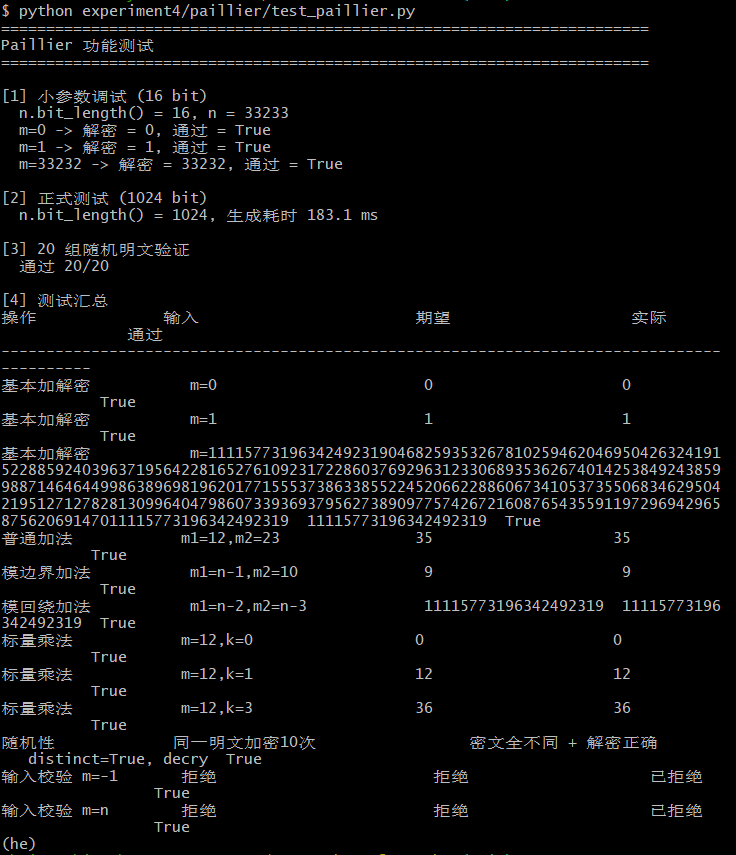
\includegraphics[width=0.95\textwidth]{figures/paillier_test.png}
  \caption{Paillier 功能测试输出}
  \label{fig:paillier_test}
\end{figure}

\subsection{phe 库对照}
使用 phe 生成 1024 bit 密钥，对 $0 \sim 1000$ 的整数执行加解密、同态加法和
标量乘法。自行实现与 phe 的解密结果完全一致。两组实现的密钥和密文格式不同，
只比较解密结果。

\begin{figure}[htbp]
  \centering
  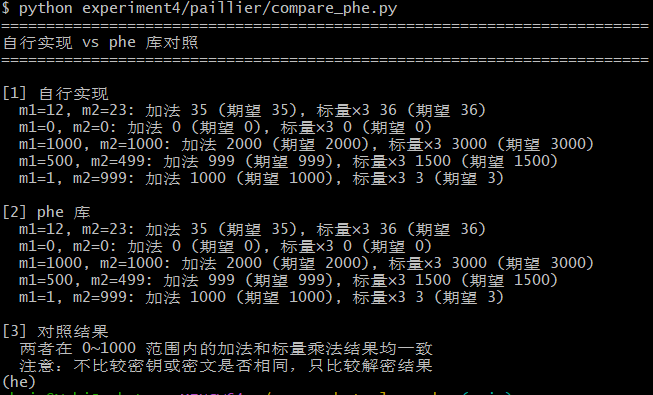
\includegraphics[width=0.95\textwidth]{figures/paillier_phe.png}
  \caption{自行实现与 phe 库对照}
  \label{fig:phe}
\end{figure}

\subsection{性能测量}
使用 512、1024、2048 bit 三种模数长度，每种独立生成 3 次密钥取中位数；
固定 20 对 $0 \sim 1000$ 的整数，预热后重复 5 轮取中位数。

\begin{table}[htbp]
\centering
\caption{Paillier 性能对比（毫秒）}
\begin{tabular}{llcccccc}
\toprule
实现 & 模数 bit & n.bit & keygen & 加密 & 加法 & 解密 & 密文/B \\
\midrule
自行 & 512 & 512 & 13.00 & 1.585 & 0.003 & 1.512 & 128 \\
phe & 512 & 512 & 8.24 & 1.545 & 0.004 & 0.556 & 128 \\
自行 & 1024 & 1024 & 78.05 & 10.759 & 0.011 & 10.891 & 256 \\
phe & 1024 & 1024 & 108.77 & 10.414 & 0.013 & 3.046 & 256 \\
自行 & 2048 & 2048 & 766.58 & 76.184 & 0.035 & 76.526 & 512 \\
phe & 2048 & 2048 & 285.66 & 76.885 & 0.038 & 21.282 & 512 \\
\bottomrule
\end{tabular}
\end{table}

\begin{figure}[htbp]
  \centering
  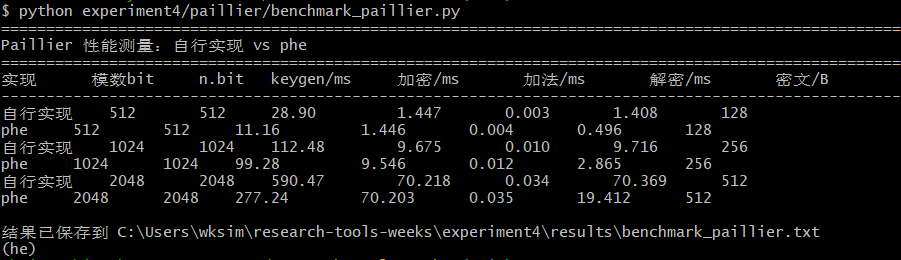
\includegraphics[width=0.95\textwidth]{figures/paillier_bench.png}
  \caption{Paillier 性能测量输出}
  \label{fig:bench}
\end{figure}

分析：加密时间两组实现接近；同态加法都是模乘，非常快；
phe 的解密明显更快，因为它内部使用 CRT 优化了解密时的模幂运算。
密钥生成时间随模数增长显著，2048 bit 时自行实现较慢。

\section{BFV 图像检索}

\subsection{BFV 运算流程}

\begin{figure}[htbp]
\centering
\begin{tikzpicture}[
    node distance=0.5cm and 0.9cm,
    box/.style={rectangle, draw, rounded corners, minimum height=0.7cm,
                minimum width=2.6cm, align=center, font=\small},
    client/.style={box, fill=blue!10},
    server/.style={box, fill=orange!15},
    arrow/.style={->, thick}
]
\node[client] (keygen) {客户端\\生成密钥};
\node[client, below=of keygen] (enc) {加密图库\\与查询};
\node[client, below=2.4cm of enc] (dec) {解密得分\\MSE = SSE/d};
\node[client, below=of dec] (rank) {排序\\返回结果};

\node[server, right=2.5cm of enc] (recv) {接收公开\\上下文+密文};
\node[server, below=of recv] (sub) {密文相减\\$c_x - c_y$};
\node[server, below=of sub] (sq) {逐元素平方\\$(c_x-c_y)^2$\\（深度 1）};
\node[server, below=of sq] (sum) {槽位求和\\（Galois）};
\node[server, below=of sum] (send) {返回得分\\密文};

\draw[arrow] (keygen) -- (enc);
\draw[arrow] (enc) -- node[above, font=\tiny]{密文} (recv);
\draw[arrow] (recv) -- (sub);
\draw[arrow] (sub) -- (sq);
\draw[arrow] (sq) -- (sum);
\draw[arrow] (sum) -- (send);
\draw[arrow] (send) -- node[above, font=\tiny]{得分密文} (dec);
\draw[arrow] (dec) -- (rank);

\node[draw, dashed, red, font=\tiny, right=0.3cm of keygen, align=left]
     {私钥\\仅客户端};
\node[draw, dashed, red, font=\tiny, right=0.3cm of send, align=left]
     {无私钥};
\end{tikzpicture}
\caption{BFV 密文图像检索流程与乘法深度}
\label{fig:flow}
\end{figure}

如图 \ref{fig:flow} 所示，密文乘法只有一层（逐元素平方），不涉及自举。
槽位求和依赖 Galois 密钥，密文乘法依赖重线性化密钥。

\subsection{明文基准}
图库 G01$\sim$G06 与查询 Q01$\sim$Q03 预处理为 4096 维向量后，
明文 SSE 距离与排名如下。

\begin{table}[htbp]
\centering
\caption{明文基准距离与排名（SSE）}
\begin{tabular}{lcccccc}
\toprule
查询 & 1st & 2nd & 3rd & 4th & 5th & 6th \\
\midrule
Q01 & G01(0) & G03(24536109) & G02(27357064) & G04(36584198) & G06(36591763) & G05(58716110) \\
Q02 & G01(419644) & G03(24322827) & G02(28431320) & G06(35581737) & G04(41200376) & G05(66738476) \\
Q03 & G03(4672723) & G02(14110992) & G04(17858010) & G06(20571819) & G01(20804484) & G05(42039986) \\
\bottomrule
\end{tabular}
\end{table}

Q01 为 G01 的副本，SSE = 0，符合预期。Q02 为 G01 的亮度/噪声扰动版本，
最近邻仍为 G01。Q03 为未入库草地纹理，最近邻为 G03（猫图），
由实测距离确定。黑图与白图 SSE = 4096 $\times$ 255$^2$ = 266342400。

\subsection{四维手算}
令 $a = (1,2,3,4)$，$b = (4,3,2,1)$：
$$a - b = (-3,-1,1,3), \quad (a-b)^2 = (9,1,1,9),$$
$$\mathrm{SSE} = 20.$$
在密文上执行相同运算，客户端解密后得到 SSE = 20，与手算一致。

\subsection{密文检索结果}

\begin{table}[htbp]
\centering
\caption{BFV 配置 A 与配置 B 的性能与正确性}
\begin{tabular}{lcccc}
\toprule
指标 & 配置 A ($N=8192$) & 配置 B ($N=16384$) \\
\midrule
系数模数总位数 & 218 & 438 \\
上下文生成 / ms & 418.2 & 3090.0 \\
上下文序列化+恢复 / ms & 638.9 & 3838.8 \\
图像加密（9 张） / ms & 66.9 & 144.8 \\
Q01 单查询遍历 / ms & 364.9 & 1997.0 \\
Q02 单查询遍历 / ms & 361.1 & 2017.1 \\
Q03 单查询遍历 / ms & 370.5 & 1974.3 \\
最大整数误差 & 0 & 0 \\
排名一致率 & 3/3 & 3/3 \\
服务器上下文无私钥 & 是 & 是 \\
black vs white 密文 SSE & 266342400 & 266342400 \\
\bottomrule
\end{tabular}
\end{table}

\begin{figure}[htbp]
  \centering
  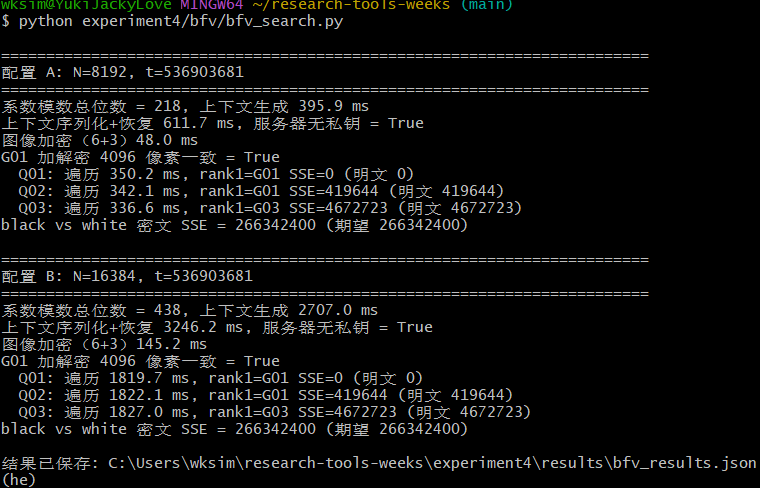
\includegraphics[width=0.95\textwidth]{figures/bfv_search.png}
  \caption{BFV 密文检索输出}
  \label{fig:bfv}
\end{figure}

分析：配置 B 的 $N$ 是配置 A 的两倍，系数模数总位数从 218 增至 438，
上下文生成时间约 7 倍，单查询遍历时间约 5.5 倍。该差异不能单独归因于 $N$，
还包括系数模数总位数增加带来的运算量和序列化开销。

\subsection{细粒度性能测量}

对配置 A、B 分别进行 5 轮预热计时，记录平均单次耗时与序列化字节大小。

\begin{table}[htbp]
\centering
\caption{BFV 细粒度性能（5 轮中位数）}
\begin{tabular}{lcc}
\toprule
指标 & 配置 A ($N=8192$) & 配置 B ($N=16384$) \\
\midrule
上下文生成 / ms & 391.0 & 2748.7 \\
上下文序列化 / ms & 264.7 & 1449.9 \\
上下文大小 / MiB & 52.21 & 425.71 \\
服务器上下文恢复 / ms & 265.4 & 1853.8 \\
图像加密（单张）/ ms & 5.163 & 15.106 \\
图像密文大小 / B & 432460 & 1825839 \\
反序列化（单对）/ ms & 2.099 & 6.666 \\
密文求值（单对）/ ms & 48.076 & 280.260 \\
得分序列化 / ms & 1.616 & 4.612 \\
得分密文大小 / B & 432538 & 1825643 \\
单查询遍历（6 图库）/ ms & 336.0 & 1828.3 \\
\bottomrule
\end{tabular}
\end{table}

\begin{figure}[htbp]
  \centering
  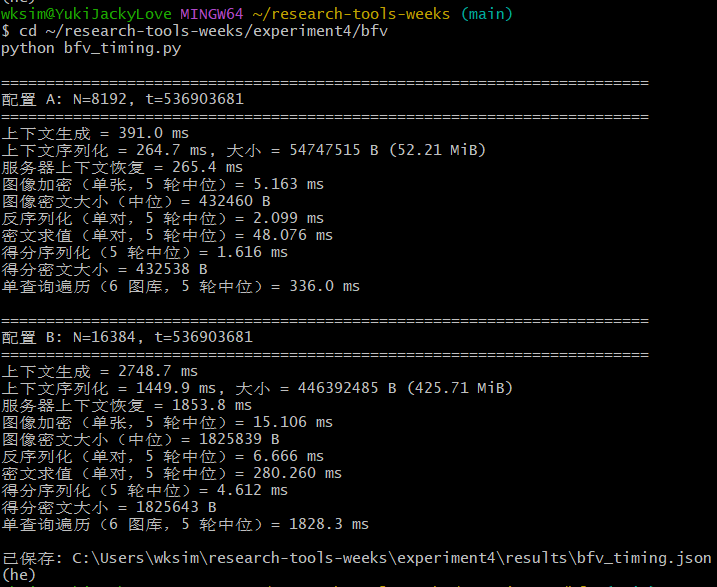
\includegraphics[width=0.95\textwidth]{figures/bfv_timing.png}
  \caption{BFV 细粒度性能测量输出}
  \label{fig:timing}
\end{figure}

配置 B 的上下文大小约为配置 A 的 8.2 倍，密文大小约为 4.2 倍，
单对求值时间约为 5.8 倍。上下文生成和恢复时间差异更大，
与系数模数总位数从 218 增至 438 直接相关。

\section{模数边界对照}

固定 $N = 8192$，将明文模数改为 $t = 65537$，用黑白极值输入。

\begin{itemize}
  \item 真实 SSE = 266342400
  \item $266342400 \bmod 65537 = 32$
  \item 有符号代表值 = 32
  \item 密文解密结果 = 32
\end{itemize}

解密结果与真实距离不同，但等于预期有符号模值，符合模运算预期。
说明当距离超过 $t/2$ 时，明文结果发生回绕。

\begin{figure}[htbp]
  \centering
  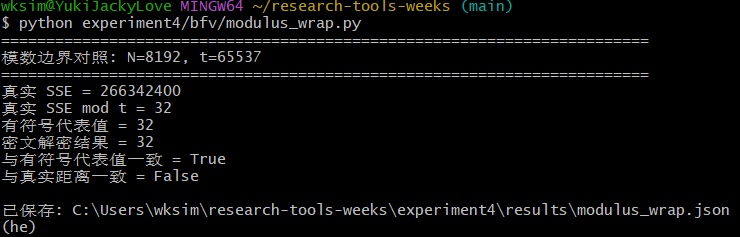
\includegraphics[width=0.9\textwidth]{figures/modulus_wrap.png}
  \caption{模数边界对照输出}
  \label{fig:wrap}
\end{figure}

\section{定点编码对照}

将灰度像素归一化为 $z_i = x_i / 255$，使用缩放因子 $K$ 转为整数
$u_i = \mathrm{rint}(K z_i)$，分别取 $K = 16, 64, 255$。

\begin{table}[htbp]
\centering
\caption{定点编码对照}
\begin{tabular}{cccc}
\toprule
$K$ & 整数误差 & 归一化 MSE 最大偏差 & 排名一致 \\
\midrule
16 & 0 & 0.003509 & 3/3 \\
64 & 0 & 0.001785 & 3/3 \\
255 & 0 & 0.000000 & 3/3 \\
\bottomrule
\end{tabular}
\end{table}

对于 $K = 512$：
$$d K^2 = 4096 \times 512^2 = 1073741824 > t/2 = 268451840.5,$$
超出有符号解码范围，会发生明文回绕，不满足恢复条件。

\begin{figure}[htbp]
  \centering
  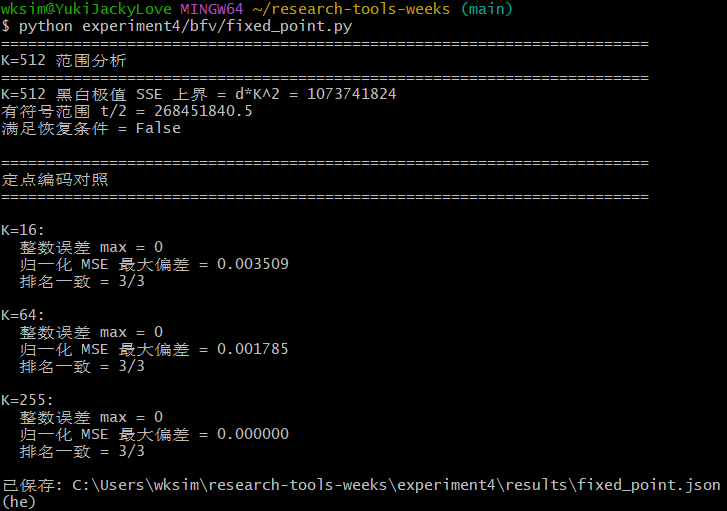
\includegraphics[width=0.9\textwidth]{figures/fixed_point.png}
  \caption{定点编码对照输出}
  \label{fig:fix}
\end{figure}

单像素舍入误差界：
$$\left| z_i - \frac{u_i}{K} \right| \le \frac{1}{2K}.$$
$K$ 越大，量化误差越小；但 $K$ 过大时整数距离上界 $dK^2$ 会超过 $t/2$，
导致明文回绕。因此 $K$ 的选择需要在量化精度和明文范围之间权衡。

\section{结果分析}

\subsection{打包编码与槽位求和}
BFV 批量编码要求 $t \equiv 1 \pmod{2N}$，两组配置均满足。
逐槽平方后使用槽位求和将 $N$ 个槽位的平方差累加为一个整数，
得到密文 SSE。求和过程使用 Galois 密钥完成旋转操作。

\subsection{评估密钥的作用}
重线性化密钥（relin keys）用于密文乘法后降低密文规模，
Galois 密钥用于槽位旋转，从而支持槽位求和。
两组密钥都是一次生成、多次使用。

\subsection{误差与异常区分}
\begin{itemize}
  \item \textbf{量化误差}：定点编码引入，与 $K$ 成反比，不会导致回绕；
  \item \textbf{明文回绕}：整数距离超过 $t/2$ 时发生，
        解密结果等于有符号模值，不等于真实距离；
  \item \textbf{计算异常}：噪声增长过大导致解密错误，
        表现为解密值与预期模值都不同。
\end{itemize}

本实验中，配置 A/B 在整数距离下误差为 0；
模数边界对照展示明文回绕；定点编码的整数误差也为 0，
归一化 MSE 偏差来自量化，符合预期。

\subsection{参数比较的控制条件}
两组配置的比较在相同图像、相同预处理、相同线程设置和相同实现下进行，
仅改变 $N$ 和默认系数模数。结果表明 $N$ 增大时，耗时和存储开销显著增加，
但都能无损恢复。

\section{代码提交记录}

本次实验的代码和结果已提交到 GitHub 仓库，提交历史如图 \ref{fig:gitlog} 所示。

\begin{figure}[htbp]
  \centering
  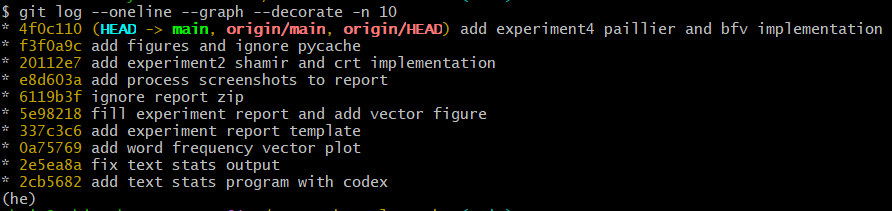
\includegraphics[width=0.95\textwidth]{figures/git_log.png}
  \caption{Git 提交历史}
  \label{fig:gitlog}
\end{figure}

\section{实验总结}
通过本次实验，我独立实现了 Paillier 部分同态加密，验证了加法同态和公开
标量乘法，并与 phe 库进行了功能和性能对照。在 BFV 部分，我实现了密文 SSE
计算电路，完成了客户端/服务器分离的图像检索流程，验证了两组参数配置下的
正确性和性能差异，并分析了明文范围、评估密钥和定点编码的作用。
实验加深了我对同态加密原理和工程实现的理解。

\end{document}